\documentclass[12pt,answers]{zjutexam}

\Year{2024--2025}
\Semester{一}
\Course{算法分析与设计}
\Type{一页开卷}

\begin{document}
\makehead
\examnotice

\begin{questions}

\question
    \fullwidth{ \textbf{判断题}( 在你认为正确的题目前的空格处写"T",错误题目前面的空格处写"F"。本题共\totalpoints 分。)}

    \begin{parts}
        \part[2]  \tf[T] 算法就是解决问题的办法。
        \part[2]  \tf[F] 快速排序算法的时间复杂度$T(n)=2T(n-1)+cn = O(n^2)$。
    \end{parts}

\question
\fullwidth{ \textbf{单项选择题}(在题目下划线处给出你认为正确选项的标号。共~\totalpoints~分)} 
  \begin{parts}
    \part [2] 你擅长\fillin。

    \begin{oneparchoices}
    \correctchoice 唱
    \correctchoice 跳
    \correctchoice RAP
    \choice 篮球
    \end{oneparchoices}

    \part  [2] 只有毫不动摇地坚持\fillin,才能实现中华民族的伟大复兴。
    \begin{choices}
    \choice 资本主义
    \choice 无政府主义
    \correctchoice 新时代中国特色社会主义
    \choice 社会主义
    \end{choices}

    \begin{solution}
    中华民族的伟大复兴需要坚持社会主义,见教材P12.
    \end{solution}
    
    \part  [2] 以下常用于求解8皇后问题的算法是什么。
    \begin{choices}
    \choice 分治算法
    \choice 分支界限
    \correctchoice 回溯算法
    \choice 动态规划
    \end{choices}

  \end{parts}


\question
    \fullwidth{ \textbf{设计题}(共\totalpoints 分)}
    \begin{parts}
        \part [10] 给出0/1背包问题的算法。
        \fillwithlines{1in}
        \begin{solution}
            0/1背包可以使用动态规划算法求解,算法的时间复杂度是$O(nS)$。\mypoints{10}
        \end{solution}
        \part [18] 设计一个贪心算法。
        \fillwithlines{2in}
        \begin{solution}
            \begin{itemize}
                \item 贪心算法。\mypoints{8}
                \item 贪心策略。\mypoints{10}
            \end{itemize}
        \end{solution}
    \end{parts}

\question[10] 简述快速排序的平均时间复杂度,并说明其最好和最坏情况下的时间复杂度。

\vspace{3cm}

\question[15] 请补全如下函数,使其输出 Fibonacci 数列第 $n$ 项。

\begin{lstlisting}[language=Python]
def fib(n):
    if n <= 1:
        ________  # (1)
    else:
        ________  # (2)

\end{lstlisting}
(1)  \underline{\hspace{2.5cm}} \mypoints{7} \\
(2)  \underline{\hspace{2.5cm}} \mypoints{6}
\begin{solution}

(1) \solutionline[5cm]{return n}{7}

(2) \solutionline[5cm]{return fib(n-1)+fib(n-2)}{8}
\end{solution}
\vspace{3cm}

\question[20] 请写出下面程序的时间复杂度(用 $T(n)$ 表示)并简化为渐进阶。

\begin{lstlisting}[language=C]
int example(int n) {
    if (n <= 1) return 1;
    return example(n/2) + example(n/2);
}
\end{lstlisting}

\question[5] 下表展示了一个背包问题的部分动态规划表格,物品重量为 $[1, 3, 4]$,价值为 $[15, 20, 30]$,背包容量为 $4$。请你完成表格并写出最大价值。

\begin{center}
\renewcommand{\arraystretch}{1.2}
\begin{tabular}{|c|c|c|c|c|c|}
\hline
物品编号 & 容量0 & 容量1 & 容量2 & 容量3 & 容量4 \\
\hline
不选任何物品 & 0 & 0 & 0 & 0 & 0 \\
\hline
选第1件 (w=1,v=15) & 0 & \underline{\hspace{1.2cm}} & \underline{\hspace{1.2cm}} & \underline{\hspace{1.2cm}} & \underline{\hspace{1.2cm}} \\
\hline
选前2件 (加上w=3,v=20) & \underline{\hspace{1.2cm}} & \underline{\hspace{1.2cm}} & \underline{\hspace{1.2cm}} & \underline{\hspace{1.2cm}} & \underline{\hspace{1.2cm}} \\
\hline
选前3件 (加上w=4,v=30) & \underline{\hspace{1.2cm}} & \underline{\hspace{1.2cm}} & \underline{\hspace{1.2cm}} & \underline{\hspace{1.2cm}} & \underline{\hspace{1.2cm}} \\
\hline
\end{tabular}
\end{center}

\vspace{0.5em}
最终最大价值为:\underline{\hspace{3cm}} \mypoints{3}
\begin{solution}
动态规划递推式:$dp[i][w] = \max(dp[i-1][w], dp[i-1][w-w_i]+v_i)$

\begin{center}
\begin{tabular}{|c|c|c|c|c|c|}
\hline
物品编号 & 容量0 & 容量1 & 容量2 & 容量3 & 容量4 \\
\hline
不选任何物品 & 0 & 0 & 0 & 0 & 0 \\
\hline
选第1件 & 0 & 15 & 15 & 15 & 15 \\
\hline
前2件 & 0 & 15 & 15 & 20 & 35 \\
\hline
前3件 & 0 & 15 & 15 & 20 & 35 \\
\hline
\end{tabular}
\end{center}

最大价值为:\underline{35} \mypoints{3}
\end{solution}

\question[5] 如下图所示为一个加权有向图。请使用 Dijkstra 算法求出从顶点 $A$ 到所有其他点的最短路径距离。

\begin{center}
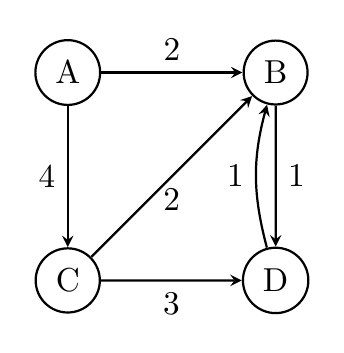
\begin{tikzpicture}[->, >=stealth, node distance=2.2cm, thick, scale=1.2, every node/.style={transform shape}]
\node[circle,draw](A){A};
\node[circle,draw,right of=A](B){B};
\node[circle,draw,below of=A](C){C};
\node[circle,draw,below of=B](D){D};

\path (A) edge node[above] {2} (B);
\path (A) edge node[left] {4} (C);
\path (B) edge node[right] {1} (D);
\path (C) edge node[below] {3} (D);
\path (C) edge node[below] {2} (B);
\path (D) edge [bend left=15] node[left] {1} (B);
\end{tikzpicture}
\end{center}

\vspace{0.5em}

请填写从 $A$ 到 $B,C,D$ 的最短路径长度:

\vspace{0.5em}

$A \to B$:\underline{\hspace{2cm}} \mypoints{3} \\
$A \to C$:\underline{\hspace{2cm}} \mypoints{3} \\
$A \to D$:\underline{\hspace{2cm}} \mypoints{4}

\begin{solution}
从 $A$ 出发使用 Dijkstra 算法:

\begin{itemize}
\item $A \to B$: 距离为 2
\item $A \to C$: 距离为 4
\item $A \to D$: $A \to B \to D$,距离为 $2 + 1 = 3$
\end{itemize}

\vspace{0.5em}

$A \to B$:\underline{2} \mypoints{3} \\
$A \to C$:\underline{4} \mypoints{3} \\
$A \to D$:\underline{3} \mypoints{4}
\end{solution}

\end{questions}
\end{document}